%%%%%%%%%%%%%%%%%%%%%%%%%%%%%%%%%%%%%%%%%%%%%%%%%%%
% PRESENTATION FOR TOM HEATON'S VISIT (11-07-2018)
% 
% Prithvi Thakur
% Geophysics research group
% Department of Earth and Environmental Science
% University of Michigan, Ann Arbor
%%%%%%%%%%%%%%%%%%%%%%%%%%%%%%%%%%%%%%%%%%%%%%%%%%%

\documentclass{beamer}

\mode<presentation> {
\usetheme{AnnArbor}
}

\usepackage{graphicx} % Allows including images
\usepackage{booktabs} % Allows the use of \toprule, \midrule and \bottomrule in tables
%\usepackage[export]{adjustbox} % To change the default alignment of image
\usepackage{subcaption} % Add subfigures to place figures side by side

%------------------------------------------------
%           TITLE PAGE INFORMATION
%------------------------------------------------
\title[MFD in EQ Cycles]{Fully Dynamic Simulations of Earthquake Cycle on a 2D Strike-Slip Fault Surrounded by Damaged Zones} 
\author{Prithvi Thakur}
\institute[UofM]
{
Research Advisor: Yihe Huang \\
\medskip
University of Michigan \\ % Your institution for the title page
\medskip
\textit{prith@umich.edu} % Your email address
}
\date{\today} % Date, can be changed to a custom date
%------------------------------------------------

%%%%%%%%%%%%%%%%
\begin{document}

% TITLE PAGE
\begin{frame}
    \titlepage 
\end{frame}

% TABLE OF CONTENTS
\begin{frame}
    \frametitle{Overview}
    \begin{itemize}
        \item 2D Numerical simulation of long-term fault slip using a spectral element method. Fully dynamic scheme for nucleation, rupture propagation, and postseismic deformation integrated with the aseismic phase. 
        \item Strike-slip fault with mode III rupture (e.g., San Andreas), surrounded by a narrow damaged zone
            of low rigidity (Fault Zone).
        \item Complex slip pattern with multiple earthquakes of various magnitudes. A characteristic type magnitude-frequency distribution observed in simulations with narrow fault zones.
    \end{itemize}
\end{frame}

% FAULT ZONE GEOMETRY
\section{Fault Zone Properties}
\begin{frame}
    \frametitle{Damaged Fault Zone Geometry}
    \begin{figure}
        \includegraphics[width=0.9\linewidth]{images/fault_zone1.png}
    \end{figure}
\end{frame}
\begin{frame}
    \frametitle{Material Properties of Observed Fault Zones}
    \begin{figure}
        \includegraphics[width=0.9\linewidth]{images/faultzonetable.png}
    \end{figure}
\end{frame}

% OBSERVATIONS: PARKFIELD MFD PLOTS
\section{Natural Observations}
\begin{frame}
    \frametitle{Observations from San-Andreas Fault}
    \begin{figure}
        \includegraphics[width=\textwidth]{images/seismicitydepth.png} 
    \end{figure}
\end{frame}
\begin{frame}
    \frametitle{Observations from San-Andreas Fault}
    \begin{figure}
        \includegraphics[width=\textwidth]{images/mfd_complete} 
    \end{figure}
\end{frame}

% MODEL DESCRIPTION
\section{Model Description}
\begin{frame}
    \frametitle{Model Description}
    \begin{figure}
        \includegraphics[width=0.9\linewidth]{images/model_setup}
    \end{figure}
\end{frame}

% RESULTS PLOT
\section{Simulated Results}
\begin{frame}
    \frametitle{Simulated Results: Homogeneous Medium}
    \begin{figure}
        \includegraphics[width=0.9\linewidth]{images/cumslipHomo.png} 
    \end{figure}
\end{frame}

\begin{frame}
    \frametitle{Simulated Results: 8 km Deep, 1.5 km Wide Fault Zone}
    \begin{figure}
        \begin{subfigure}[b]{0.5\textwidth}
            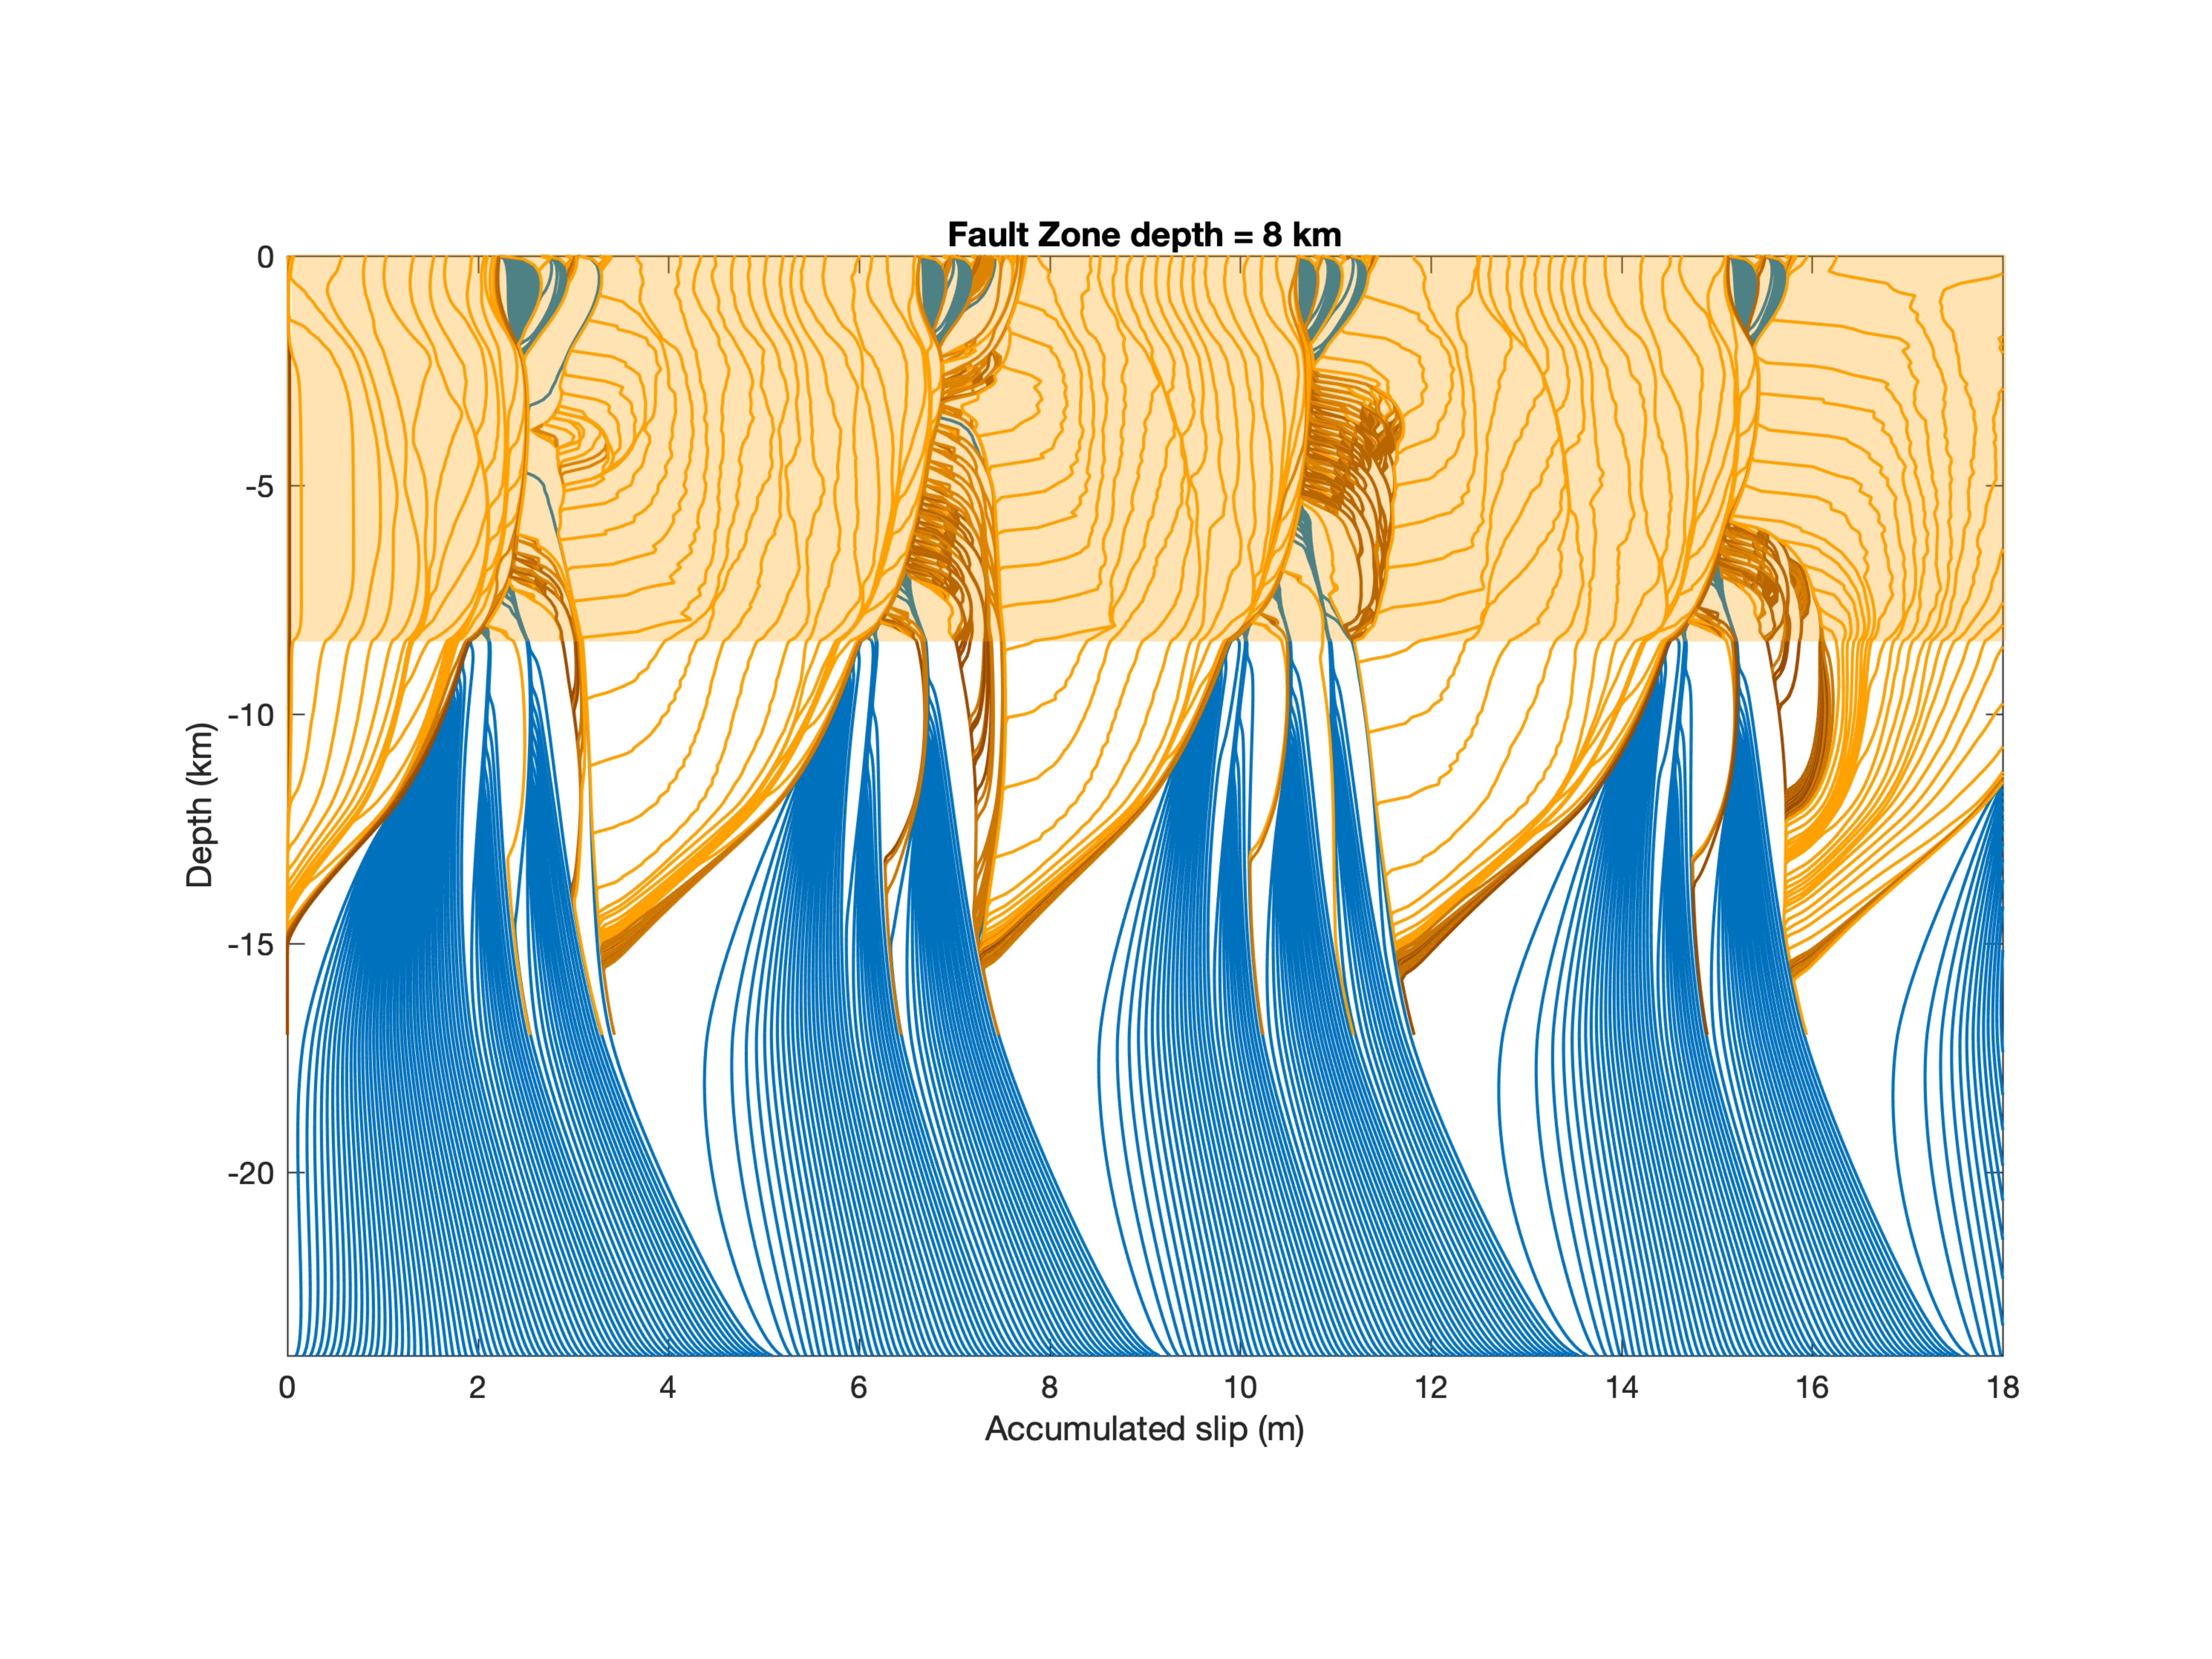
\includegraphics[width=\textwidth]{images/untitled.png} 
        \end{subfigure}%
        \begin{subfigure}[b]{0.5\textwidth}
            \includegraphics[width=\textwidth]{images/catalogue.jpg}
        \end{subfigure}%
    \end{figure}
\end{frame}
\begin{frame}
    \frametitle{Simulated Results: MFD and Earthquake Location}
    \begin{figure}
        \begin{subfigure}[b]{0.5\textwidth}
            \includegraphics[width=\textwidth]{images/hypocenter1.png} 
        \end{subfigure}%
        \begin{subfigure}[b]{0.5\textwidth}
            \includegraphics[width=\textwidth]{images/mfd1.png}
        \end{subfigure}%
    \end{figure}
\end{frame}


% CONCLUSIONS
\section{Conclusions}
\begin{frame}
    \frametitle{Conclusions}
    \begin{itemize}
        \item The presence of fault zone promotes stress heterogeneity.
        \item This stress heterogeneity gives rise to a power law distribution of earthquakes.
        \item The distribution is more similar to characteristic type earthquake distribution.
        \item Earthquake cycle simulations with dynamic treatment of inertial effects gives a more realistic view of earthquake distribution in the presence of a material heterogeneity.
        \end{itemize}
\end{frame}

% FUTURE WORK
\section{Future Work}
\begin{frame}
    \frametitle{Future Work}
    \includegraphics[width=\textwidth]{images/model_setup_scec.png} 
\end{frame}

% ENDING SLIDE
\begin{frame}
    \Huge{\centerline{That's All Folks!!}}
\end{frame}
\end{document} 
%%%%%%%%%%%%%%%%
